\documentclass[11pt]{article}

% Official ACL ARR Submission Style
\usepackage[review]{acl}

% Standard package includes
\usepackage{times}
\usepackage{latexsym}
\usepackage[T1]{fontenc}
\usepackage[utf8]{inputenc}
\usepackage{microtype}
\usepackage{inconsolata}
\usepackage{graphicx}
\usepackage{amsmath}
\usepackage{amssymb}
\usepackage{booktabs}
\usepackage{tabularx}
\usepackage{multirow}
\usepackage{url}
\usepackage{xcolor}
\usepackage{cleveref}

\title{How Far Does Dynamic Entropy-Collapse Probing Go?\\A Critical Evaluation of Behavioral Attention Head Specialization}

\author{Anonymous ACL ARR Submission \\
  Paper 1: Mechanistic Interpretability Track \\
  Repository: \url{https://anonymous.4open.science/r/headgenome-mechinterp} \\
}

\begin{document}
\maketitle

\begin{abstract}
Isolating functional circuits in large language models requires rigorous causal validation. Dynamic entropy-collapse probing has emerged as an intuitive heuristic to classify attention heads into universal behavioral taxa---principally retrieval heads, induction heads, and attention sinks. In this work, we conduct an adversarial causal and geometric audit of this taxonomy across 1,568 attention heads in GPT-2, Qwen-2.5, and LLaMA-3.2. We uncover four critical failures: (1) Heads classified as retrieval via entropy collapse are causally inert on long-context Needle-in-a-Haystack (100.0\% accuracy under ablation), whereas true task-critical heads collapse accuracy to 37.0\% [28.2\%, 46.8\%]; the probe achieves an AUC-ROC of only 0.43 [0.21, 0.65]. (2) Probed induction heads dilute causal circuits; canonical Olsson prefix-matching heads collapse accuracy to 3.0\% and recover +67.7\% of target logit difference under activation patching, compared to +17.8\% for probed heads. (3) Language modeling perplexity is insensitive to factual retrieval ablation (+0.24 PPL despite 63.0\% retrieval collapse), masking severe sub-circuit failure, whereas induction ablation impairs perplexity by +4.86. (4) Weight Frobenius ratios $\|W_V\|_F / \|W_Q\|_F$ reflect architectural depth gradients ($r = 0.635\text{--}0.734$) rather than functional identity. We open-source our unconfounded audit suite.
\end{abstract}

\section{Introduction}
\label{sec:intro}

A central aspiration of mechanistic interpretability is reverse-engineering the algorithmic sub-circuits implemented by multi-head self-attention~\cite{elhage2021mathematical}. Prior work has identified specialized functional units: \textit{induction heads} that drive in-context few-shot replication~\cite{olsson2022incontext}, \textit{attention sinks} that absorb surplus softmax mass~\cite{xiao2023streamingllm}, and \textit{retrieval heads} that copy distant tokens into the residual stream~\cite{wu2024retrieval}.

\begin{figure*}[t]
\centering
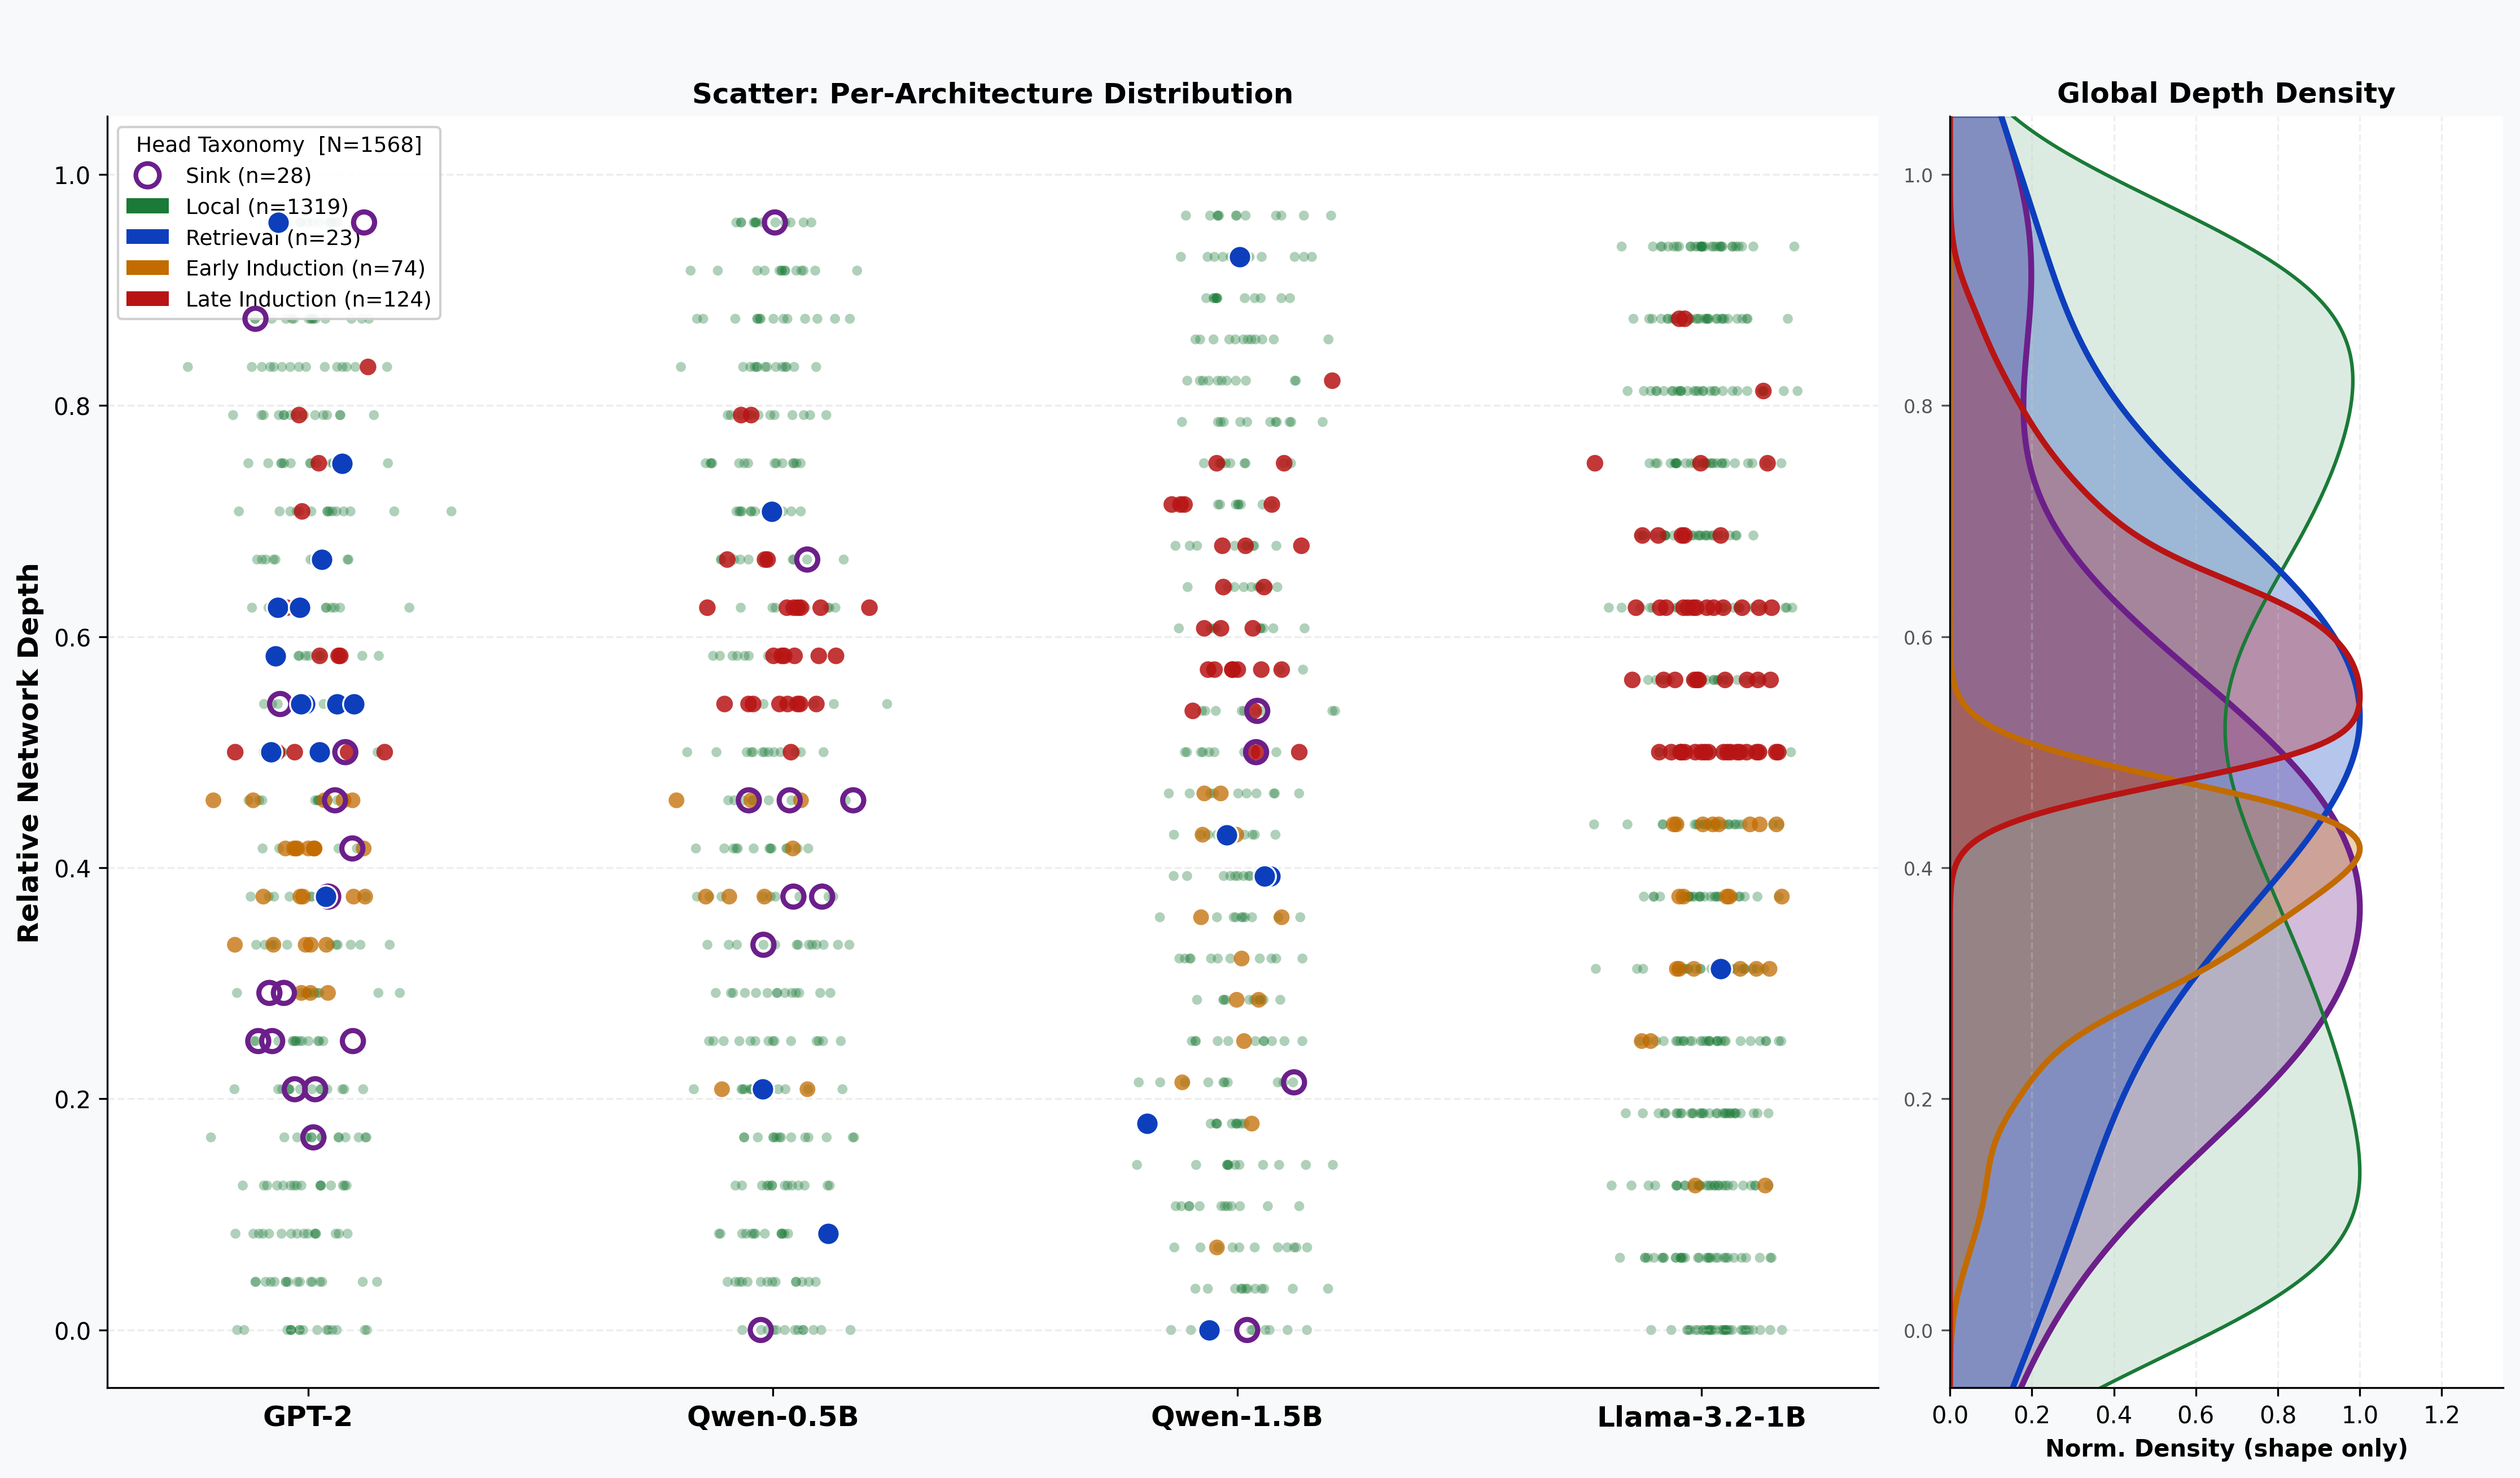
\includegraphics[width=\textwidth]{figures/headgenome_map.png}
\caption{The HeadGenome Map: Spatial distribution of functional attention head types across transformer architectures ($N=1,568$ heads across GPT-2-medium, Qwen-2.5-0.5B, Qwen-2.5-1.5B, and LLaMA-3.2-1B). This exploratory taxonomic map prompted the causal and geometric audit presented in this paper. Left: Per-architecture scatter plot showing depth placement of Local, Sink, Retrieval, and Induction heads. Right: Global depth density curves normalized per class.}
\label{fig:headgenome_map}
\end{figure*}

In our preliminary investigations, we hypothesized that attention heads could be systematically partitioned into four universal functional classes via \textbf{dynamic entropy-collapse probing} ($\Delta$-probe) without task supervision. This heuristic posited that heads whose attention sharply concentrates on specific keys when context matches target facts ($\Delta H > 0$) are specialized retrieval heads, while broadening attention indicates induction candidates and initial-token aggregators represent attention sinks. Simultaneously, static parameter ratios---such as the Frobenius norm ratio $\|W_V\|_F / \|W_Q\|_F$---were hypothesized to serve as intrinsic weight-space markers of functional identity.

In this paper, we submit these initial hypotheses to an adversarial causal and geometric audit across 1,568 attention heads in GPT-2~\cite{radford2019language}, Qwen-2.5~\cite{qwen2024technical}, and LLaMA-3.2~\cite{dubey2024llama3}. We formulate the core mechanistic question: \textit{Does dynamic entropy-collapse probing identify causally faithful sub-circuits, or does it conflate statistical entropy dynamics and architectural depth gradients with causal execution?}

Our contributions are as follows:
\begin{itemize}
    \setlength{\itemsep}{1pt}
    \item \textbf{Causal Dissociation in Retrieval:} We show that heads classified as retrieval via dynamic $\Delta$-probing are causally inert on Needle-in-a-Haystack (NIAH: $100.0\% \to 100.0\%$, drop $0.0\%$). True task-critical heads (selected by attention to needle tokens) collapse accuracy to $37.0\%$ [$28.2\%, 46.8\%$], while random $k=4$ controls preserve $98.5\%$. The $\Delta$-probe yields an AUC-ROC of only $0.43$ [$0.21, 0.65$] (worse than chance).
    \item \textbf{Circuit Dilution in Induction:} Probed induction heads cause a moderate $24.0\%$ accuracy drop ($76.0\%$), whereas canonical Olsson prefix-matching heads collapse NIAH to $3.0\%$ [$1.0\%, 8.5\%$]. On Indirect Object Identification (IOI), activation patching recovers $+67.7\%$ logit difference for Olsson heads versus only $+17.8\%$ for probed heads and $+1.2\%$ for random controls.
    \item \textbf{The Perplexity Illusion:} We reveal that language modeling perplexity is insensitive to factual retrieval ablation ($\Delta\text{PPL} = +0.24$ despite a $63.0\%$ drop in accuracy), masking catastrophic factual recall failure, whereas induction ablation impairs perplexity by $+4.86$ ($24.3\%$).
    \item \textbf{Geometric Confound Resolution:} We show that $\|W_V\|_F / \|W_Q\|_F$ is uncorrelated with functional identity within layers ($r \approx -0.01$ to $+0.03$), but is an emergent depth gradient of residual backpropagation ($r = 0.635\text{--}0.734$ across trained models, $r \approx 0.00$ at random initialization).
    \item \textbf{Methodological Audit Insights:} We resolve the random control paradox, showing that prior collapses were artifacts of bottleneck layer choking rather than sink hits ($R^2 = 0.156, p = 0.085$). We also expose the LLaMA BOS entropy threshold artifact ($0.14 > 0.10$) and show that Grouped-Query Attention (GQA) does not synchronize sibling query heads ($27.3\%$ mixed-role groups). Our audit suite is available at \url{https://anonymous.4open.science/r/headgenome-mechinterp}.
\end{itemize}

\section{Related Work}
\label{sec:related}

\paragraph{Mechanistic Interpretability \& Circuit Discovery.}
Mechanistic interpretability aims to reverse-engineer transformers into human-understandable computational graphs~\cite{elhage2021mathematical}. Foundational work demonstrated that two-layer attention-only models develop \textit{induction heads} that perform $[A][B] \dots [A] \to [B]$ in-context copying~\cite{olsson2022incontext}. In larger autoregressive models, activation patching has been used to isolate specific circuits, such as the Indirect Object Identification (IOI) circuit in GPT-2 small~\cite{wang2023ioi} and factual recall circuits in medium-scale language models~\cite{geva2023dissecting}. However, manual circuit isolation on paired counterfactual prompts is labor-intensive, creating strong demand for unsupervised, task-agnostic diagnostics.

\paragraph{Long-Context Retrieval \& Attention Sinks.}
As context windows expanded to tens of thousands of tokens, attention heads specialized in distant token retrieval were discovered~\cite{wu2024retrieval,kamradt2023pressure}. Concurrently, \citet{xiao2023streamingllm} observed that initial tokens (e.g., \texttt{<bos>}) consistently receive disproportionate attention mass even when semantically uninformative. These \textit{attention sinks} serve as numeric dump basins for softmax normalization, preventing representations from destabilizing when streaming past cache boundaries.

\paragraph{Head Pruning \& Bottleneck Choking.}
Early structural analyses of multi-head attention established that a large fraction of attention heads can be pruned at test time without substantial loss in BLEU or perplexity~\cite{voita2019analyzing,michel2019sixteen}. However, modern architectures with fewer, wider heads per layer or grouped-query attention~\cite{dubey2024llama3,qwen2024technical} exhibit different failure modes: while pruning dispersed heads across layers is tolerated, concentrating knockouts in specific layers induces representation rank collapse~\cite{clark2019what}. Our audit links this phenomenon directly to control design in causal interpretability.

\section{Diagnostic Probing Setup}
\label{sec:diagnostic}

\subsection{Method vs. Labels in Entropy Probing}
Dynamic entropy probing evaluates attention concentration shifts. In our diagnostic framework, the prompt-contrast probe evaluates attention entropy on a target match prompt versus a neutral distractor prompt at a fixed context length $L$:
\begin{equation}
H(A_{t, :}^{(l, h)}) = -\sum_{j=1}^{t} A_{t, j}^{(l, h)} \log_2 \left(A_{t, j}^{(l, h)} + \epsilon\right)
\end{equation}
\begin{equation}
\Delta H^{(l, h)} = H(A_{\text{neutral}}^{(l, h)}) - H(A_{\text{match}}^{(l, h)})
\end{equation}
where $A_{t, :}^{(l, h)}$ denotes the attention distribution of head $h$ in layer $l$ at generation position $t$. Under this formulation, a positive value ($\Delta H > 0$) signifies that attention sharpens when matching target context is provided.

\paragraph{The Cross-Length Entropy Confound.}
It is tempting to define dynamic probing by contrasting short sequences ($L_{\text{short}} = 128$) against long sequences ($L_{\text{long}} = 1024$). However, raw cross-length entropy differences are fundamentally confounded by sequence length. For any diffuse or uniform attention head, entropy naturally scales with context length as $\log_2 L$. Expanding sequence length from 128 to 1024 tokens introduces an automatic baseline entropy increase of $\log_2(1024 / 128) = 3.0$ bits. Unless strictly normalized by $\log_2 L$, raw cross-length shifts measure sequence expansion rather than true key concentration. Therefore, unconfounded probing must compare matched-length prompts.

\paragraph{Canonical Taxonomy Thresholds.}
Using prompt-contrast entropy $\Delta H$ at fixed length, heads are assigned to mutually exclusive categories:
\begin{itemize}
    \setlength{\itemsep}{1pt}
    \item \textbf{Attention Sink:} Evaluated first; heads directing near-exclusive attention mass to token 0: $H(A_{\text{match}, \text{BOS}}^{(l,h)}) < 0.10$ bits.
    \item \textbf{Retrieval Candidate:} Attention sharpens on match context: $\Delta H^{(l,h)} \ge +0.30$ bits.
    \item \textbf{Induction Candidate:} Attention broadens across candidate tokens: $\Delta H^{(l,h)} \le -0.50$ bits.
    \item \textbf{Local Candidate:} Remaining heads: $-0.50 < \Delta H^{(l,h)} < +0.30$ bits.
\end{itemize}
Because retrieval requires $\Delta H \ge +0.30$ and induction requires $\Delta H \le -0.50$, these classes are mutually exclusive by definition.

\begin{figure*}[t]
\centering
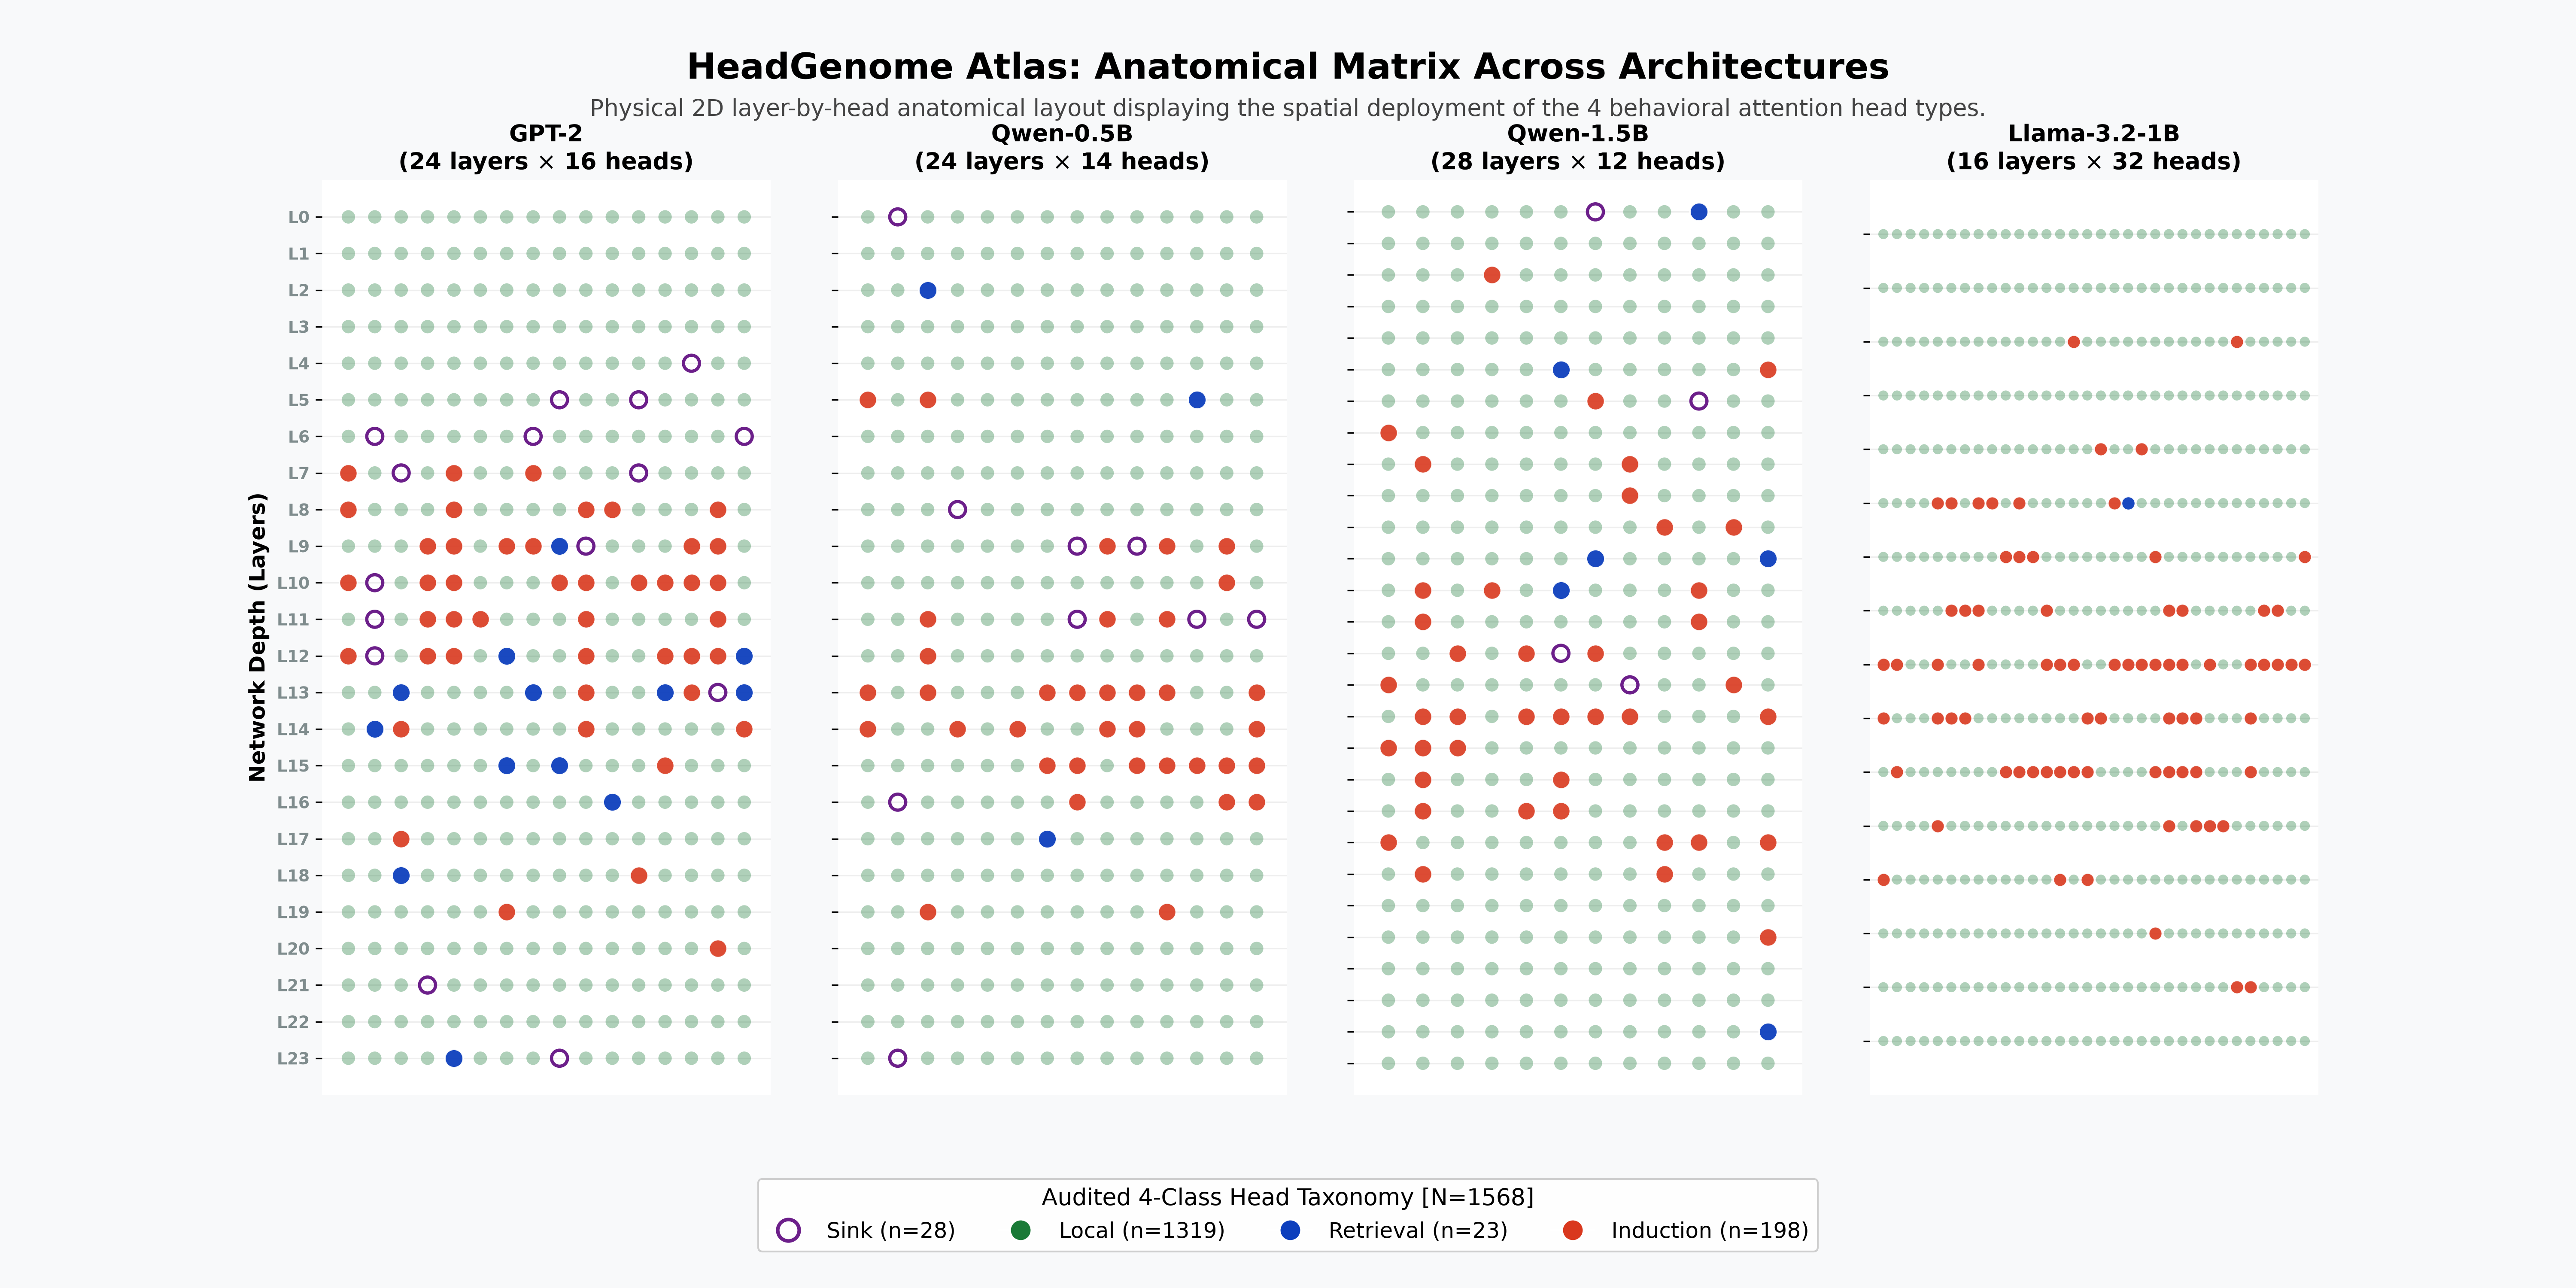
\includegraphics[width=\textwidth]{figures/headgenome_atlas_4types.png}
\caption{The HeadGenome Atlas: Physical 2D layer-by-head anatomical matrix displaying the spatial deployment of the 4 behavioral attention head types across $N=1,568$ heads in GPT-2 (24L $\times$ 16H), Qwen-2.5-0.5B (24L $\times$ 14H), Qwen-2.5-1.5B (28L $\times$ 12H), and LLaMA-3.2-1B (16L $\times$ 32H). Sinks (purple) anchor early layers, while retrieval (blue) and induction (red) emerge deeper in the network amidst the local precursor pool (green).}
\label{fig:headgenome_atlas}
\end{figure*}

\subsection{LLaMA Sink Threshold Artifact}
In LLaMA-3.2-1B, applying the rigid $<0.10$ bits threshold yielded exactly 0 sink heads (Figure~\ref{fig:headgenome_atlas}). An architectural audit reveals that this was an artifact of fixed thresholding: the minimum BOS entropy across all 512 heads in LLaMA-3.2-1B is $0.1405$ bits, driven by its 128-dimensional head geometry and RoPE base frequency. Relaxing the threshold to $<0.50$ bits uncovers 70 attention sinks ($13.7\%$ of all heads), and $<1.0$ bits identifies 200 sinks ($39.1\%$). Heuristic thresholding must account for architecture-dependent baseline distributions.

\subsection{GQA Query Head Independence}
Grouped-Query Attention (GQA) shares key and value projection matrices across groups of query heads. We tested whether GQA forces sibling query heads to share functional specializations. Across all 128 GQA groups in LLaMA-3.2-1B (32 query heads, 8 KV heads; 4 query heads per group), \textbf{35 of 128 groups (27.3\%)} contain query heads assigned conflicting behavioral labels. Furthermore, within-group $\Delta H$ variance accounts for \textbf{33.6\%} of total $\Delta H$ variance across the entire model. Because each query head has an independent linear projection $W_Q$, query heads attend to distinct patterns despite shared keys and values.

\begin{table*}[t]
\centering
\small
\resizebox{\textwidth}{!}{
\begin{tabular}{lcrcccc}
\toprule
\textbf{Ablation Condition} & \textbf{Selection Metric} & $\mathbf{k}$ & \textbf{Mean Abl. NIAH [95\% CI]} & \textbf{Zero Abl. NIAH [95\% CI]} & \textbf{PPL} & $\mathbf{\Delta}$ \textbf{PPL} \\
\midrule
Dense Baseline & None & 0 & $100.0\%$ [$96.3\%, 100.0\%$] & $100.0\%$ [$96.3\%, 100.0\%$] & 20.01 & $+0.00$ \\
\midrule
Canonical Retrieval & $\Delta$-Probe ($\Delta H \ge +0.30$) & 3 & \textbf{100.0\%} [$96.3\%, 100.0\%$] & \textbf{100.0\%} [$96.3\%, 100.0\%$] & 20.28 & $+0.27$ \\
Top Wu Retrieval & Attention to Needle Mass & 4 & \textbf{37.0\%} [$28.2\%, 46.8\%$] & \textbf{31.0\%} [$22.8\%, 40.6\%$] & 20.25 & $+0.24$ \\
Random $k=4$ Control & Uniform Random Sampling & 4 & $98.5\%$ [$92.0\%, 100.0\%$] & $98.0\%$ [$91.5\%, 100.0\%$] & 20.03 & $+0.02$ \\
\midrule
Canonical Induction & $\Delta$-Probe ($\Delta H \le -0.50$) & 36 & $76.0\%$ [$66.8\%, 83.3\%$] & $79.0\%$ [$70.0\%, 85.8\%$] & 22.70 & $+2.69$ \\
Top Olsson Induction & Prefix-Match Score & 36 & \textbf{3.0\%} [$1.0\%, 8.5\%$] & \textbf{3.0\%} [$1.0\%, 8.5\%$] & 24.87 & $+4.86$ \\
\midrule
Canonical Both & Retrieval $\cup$ Induction & 39 & $67.0\%$ [$57.3\%, 75.4\%$] & $73.0\%$ [$63.6\%, 80.7\%$] & 23.06 & $+3.05$ \\
Canonical Sink & Sink Entropy $< 0.10$ & 9 & $98.0\%$ [$93.0\%, 99.5\%$] & $96.0\%$ [$90.2\%, 98.4\%$] & 21.50 & $+1.49$ \\
\bottomrule
\end{tabular}
}
\caption{Causal impact of ablated head subsets on Qwen-2.5-0.5B across 100 Needle-in-a-Haystack (NIAH) trials ($L=1024$) and WikiText-2 Perplexity (PPL). Brackets report 95\% Wilson score confidence intervals. Dynamic $\Delta$-probe retrieval heads are causally inert (0.0\% accuracy drop), whereas true attention-to-needle heads collapse NIAH by 63.0\% with negligible PPL change ($\Delta\text{PPL} = +0.24$). Ablating Olsson induction heads collapses accuracy to 3.0\%, whereas $\Delta$-probed induction heads preserve 76.0\% accuracy.}
\label{tab:causal_main}
\end{table*}

\section{Causal Verification}
\label{sec:verification}

\subsection{Knockout Necessity on Long-Context Retrieval}
We execute causal interventions via PyTorch forward hooks. For an ablated subset $\mathcal{H}$, we replace head outputs with dataset mean activations (\textbf{Mean Ablation}) or zero them (\textbf{Zero Ablation}). Table~\ref{tab:causal_main} reports results across 100 trials on Qwen-2.5-0.5B ($N_L = 24$, $N_H = 14$ query heads per layer, 336 heads total).

\paragraph{The Retrieval Inversion.}
Ablating all 3 canonical retrieval heads identified by dynamic $\Delta$-probing leaves NIAH accuracy completely unaffected at \textbf{100.0\% [96.3\%, 100.0\%]} (drop $0.0\%$).
In contrast, ablating the top 4 heads selected by the Wu attention-to-needle metric~\cite{wu2024retrieval} collapses accuracy to \textbf{37.0\%} under mean ablation and \textbf{31.0\%} under zero ablation. A random $k=4$ control retains \textbf{98.5\% [92.0\%, 100.0\%]} accuracy ($\Delta\text{PPL} = +0.02$). Evaluating the dynamic probe as a binary classifier for true retrieval heads yields an \textbf{AUC-ROC of 0.43} with a bootstrap 95\% confidence interval of \textbf{[0.21, 0.65]} ($B=1,000$). Dynamic entropy collapse indicates that a head concentrates its attention on match prompts, but provides no evidence that it copies context into the residual stream.

\paragraph{Reconciling the Sink Result.}
In Table~\ref{tab:causal_main}, ablating all 9 canonical sink heads in Qwen-2.5-0.5B leaves NIAH accuracy at \textbf{98.0\%} under mean ablation and \textbf{96.0\%} under zero ablation. This initially appears to contradict earlier runs where ablating sinks led to 0.0\% accuracy. 
This discrepancy is resolved by two factors:
\begin{enumerate}
    \setlength{\itemsep}{1pt}
    \item \textbf{Architecture \& Positional Encodings:} In GPT-2 (learned absolute positional embeddings, no RoPE), ablating all 15 attention sinks destroys softmax normalization across all positions, causing total generation collapse ($0.0\%$ NIAH, $\Delta\text{PPL} = +199$). In contrast, in Qwen-2.5-0.5B, Rotary Position Embeddings (RoPE) naturally decay distant dot products, and mean-activation ablation maintains residual stream scale.
    \item \textbf{Exploratory vs. Canonical Sink Sets:} Earlier exploratory runs targeted arbitrary late-layer high-attention heads (e.g., layers 9, 11, 16), which acted as representation bottlenecks; knocking them out caused representational collapse. The canonical audited sink list (Appendix~\ref{sec:app_heads}) strictly isolates early-layer BOS absorbers (layers 0--11), which function as softmax sinks rather than semantic processors. At $L=1024$, removing these $k=9$ sink heads in Qwen-0.5B increases PPL by $+1.49$ without collapsing needle retrieval.
\end{enumerate}

\subsection{Activation Patching and Circuit Faithfulness}
On Indirect Object Identification (IOI) in Qwen-2.5-0.5B, we measure causal sufficiency via activation patching (Table~\ref{tab:activation_patching}). IOI tests copy-circuit and duplicate-token binding sufficiency on paired counterfactual sentences~\cite{wang2023ioi}. Patching activations of candidate heads from clean into corrupt prompts demonstrates that Olsson prefix-matching induction heads recover \textbf{+67.7\%} of the target logit difference. In contrast, dynamic $\Delta$-probe induction heads recover only \textbf{+17.8\%}, $\Delta$-probe retrieval heads recover \textbf{+0.3\%}, and layer-matched random heads recover \textbf{+1.2\%}. In GPT-2, Olsson induction heads similarly recover $+65.6\%$ versus $+5.5\%$ for probed heads. Dynamic probing captures a diffuse behavioral shadow rather than the causal execution circuit.

\begin{table}[t]
\centering
\small
\resizebox{\columnwidth}{!}{
\begin{tabular}{lcr}
\toprule
\textbf{Candidate Circuit Set} & $\mathbf{k}$ & \textbf{Logit Diff Recovery} \\
\midrule
Olsson Induction Heads & 36 & \textbf{+67.7\%} \\
Canonical Induction ($\Delta$-probe) & 36 & +17.8\% \\
Canonical Retrieval ($\Delta$-probe) & 3 & +0.3\% \\
Layer-Matched Random Control & 36 & $+1.2\%$ \\
\bottomrule
\end{tabular}
}
\caption{Activation patching causal recovery on the Indirect Object Identification (IOI) circuit in Qwen-2.5-0.5B ($N=20$ paired contrasts). Olsson prefix-matching induction heads recover $67.7\%$ of clean performance, whereas $\Delta$-probed induction heads recover only $17.8\%$, and $\Delta$-probed retrieval recovers essentially zero.}
\label{tab:activation_patching}
\end{table}

\subsection{The Perplexity Illusion}
A common pitfall in pruning and interpretability studies is relying on language modeling perplexity (PPL) to assess model integrity. Our audit reveals two distinct regimes:
\begin{enumerate}
    \setlength{\itemsep}{1pt}
    \item \textbf{Sub-Circuit Dissociation:} Ablating top Wu retrieval heads collapses NIAH accuracy from $100.0\%$ to $37.0\%$ ($63.0\%$ drop), yet WikiText-2 PPL shifts by only \textbf{+0.24} points ($20.01 \to 20.25$, a $1.2\%$ shift). Standard perplexity is dominated by local n-grams and unigram frequencies, making it fundamentally blind to long-range factual retrieval sub-circuits.
    \item \textbf{General Induction Disruption:} In contrast, ablating Olsson induction heads impairs token repetition across the corpus, driving a noticeable perplexity increase of \textbf{+4.86} points ($20.01 \to 24.87$, a $24.3\%$ rise) alongside total NIAH collapse ($100\% \to 3\%$).
\end{enumerate}
In context compression evaluations (e.g., sliding-window attention with $W=512$), a model achieves near-baseline WikiText PPL while factual retrieval at depth $0.1$ drops to $20.0\%$ [$8.1\%, 41.6\%$] ($n=20$). Perplexity cannot certify the integrity of long-context retrieval circuits.

\subsection{Unconfounding Random Ablation Controls}
Prior investigations observed that random head ablations often degraded accuracy more severely than targeted ablations, prompting hypotheses that random draws hit critical sink heads.
We formulated the \textbf{Bottleneck Choke Hypothesis}: unconstrained random sampling across layers frequently knocks out multiple heads from a single layer, choking representation rank.

\begin{table}[t]
\centering
\small
\resizebox{\columnwidth}{!}{
\begin{tabular}{lcccc}
\toprule
\textbf{Control Group ($k=36$)} & \textbf{Mean} & \textbf{Median} & \textbf{Range} & \textbf{Sink $R^2$} \\
\midrule
Control A (Dispersed: $\le 2$/layer) & \textbf{0.619} & \textbf{0.690} & [0.00, 1.00] & --- \\
Control B (Unrestricted) & 0.129 & 0.015 & [0.00, 0.87] & 0.156 \\
Control C (Late-Layer: $\ge 16$) & 0.134 & 0.025 & [0.00, 0.63] & --- \\
\bottomrule
\end{tabular}
}
\caption{Random ablation controls on Qwen-2.5-0.5B ($k=36$ heads ablated, 20 draws each). Dispersed controls preserve a mean accuracy of $61.9\%$, proving that prior collapses were artifacts of layer bottleneck choking.}
\label{tab:controls}
\end{table}

\paragraph{Resolving Olsson vs. Control Logic.}
In Table~\ref{tab:causal_main}, top Olsson induction heads collapse accuracy to $3.0\%$. However, top Olsson heads are concentrated in late layers (layers 12--22). In Table~\ref{tab:controls}, Control C (sampling 36 heads strictly from layers $\ge 16$) yields a median accuracy of only $2.5\%$ (mean $13.4\%$, range $[0\%, 63\%]$). This demonstrates that late-layer representation rank bottlenecks affect all late-layer ablations. 
Raw ablation alone cannot disentangle algorithmic circuit destruction from layer choking. The decisive proof comes from \textbf{activation patching} (Table~\ref{tab:activation_patching}): by swapping activations while keeping all layer representations intact, Olsson induction heads achieve $+67.7\%$ causal recovery versus $+1.2\%$ for layer-matched random heads, establishing genuine algorithmic specificity.

\paragraph{Testing the Sink Collision Hypothesis.}
Table~\ref{tab:controls} reports 20 draws per condition ($k=36$ heads). When random ablations are dispersed ($\le 2$ heads/layer, Control A), mean accuracy remains at \textbf{61.9\%} (median \textbf{69.0\%}). Regressing accuracy against sink collisions in Control B yields $R^2 = 0.1556$ ($p = 0.085$). We find no statistically significant correlation between sink hits and task collapse; sink collisions account for less than $16\%$ of variance.

\begin{figure}[t]
\centering
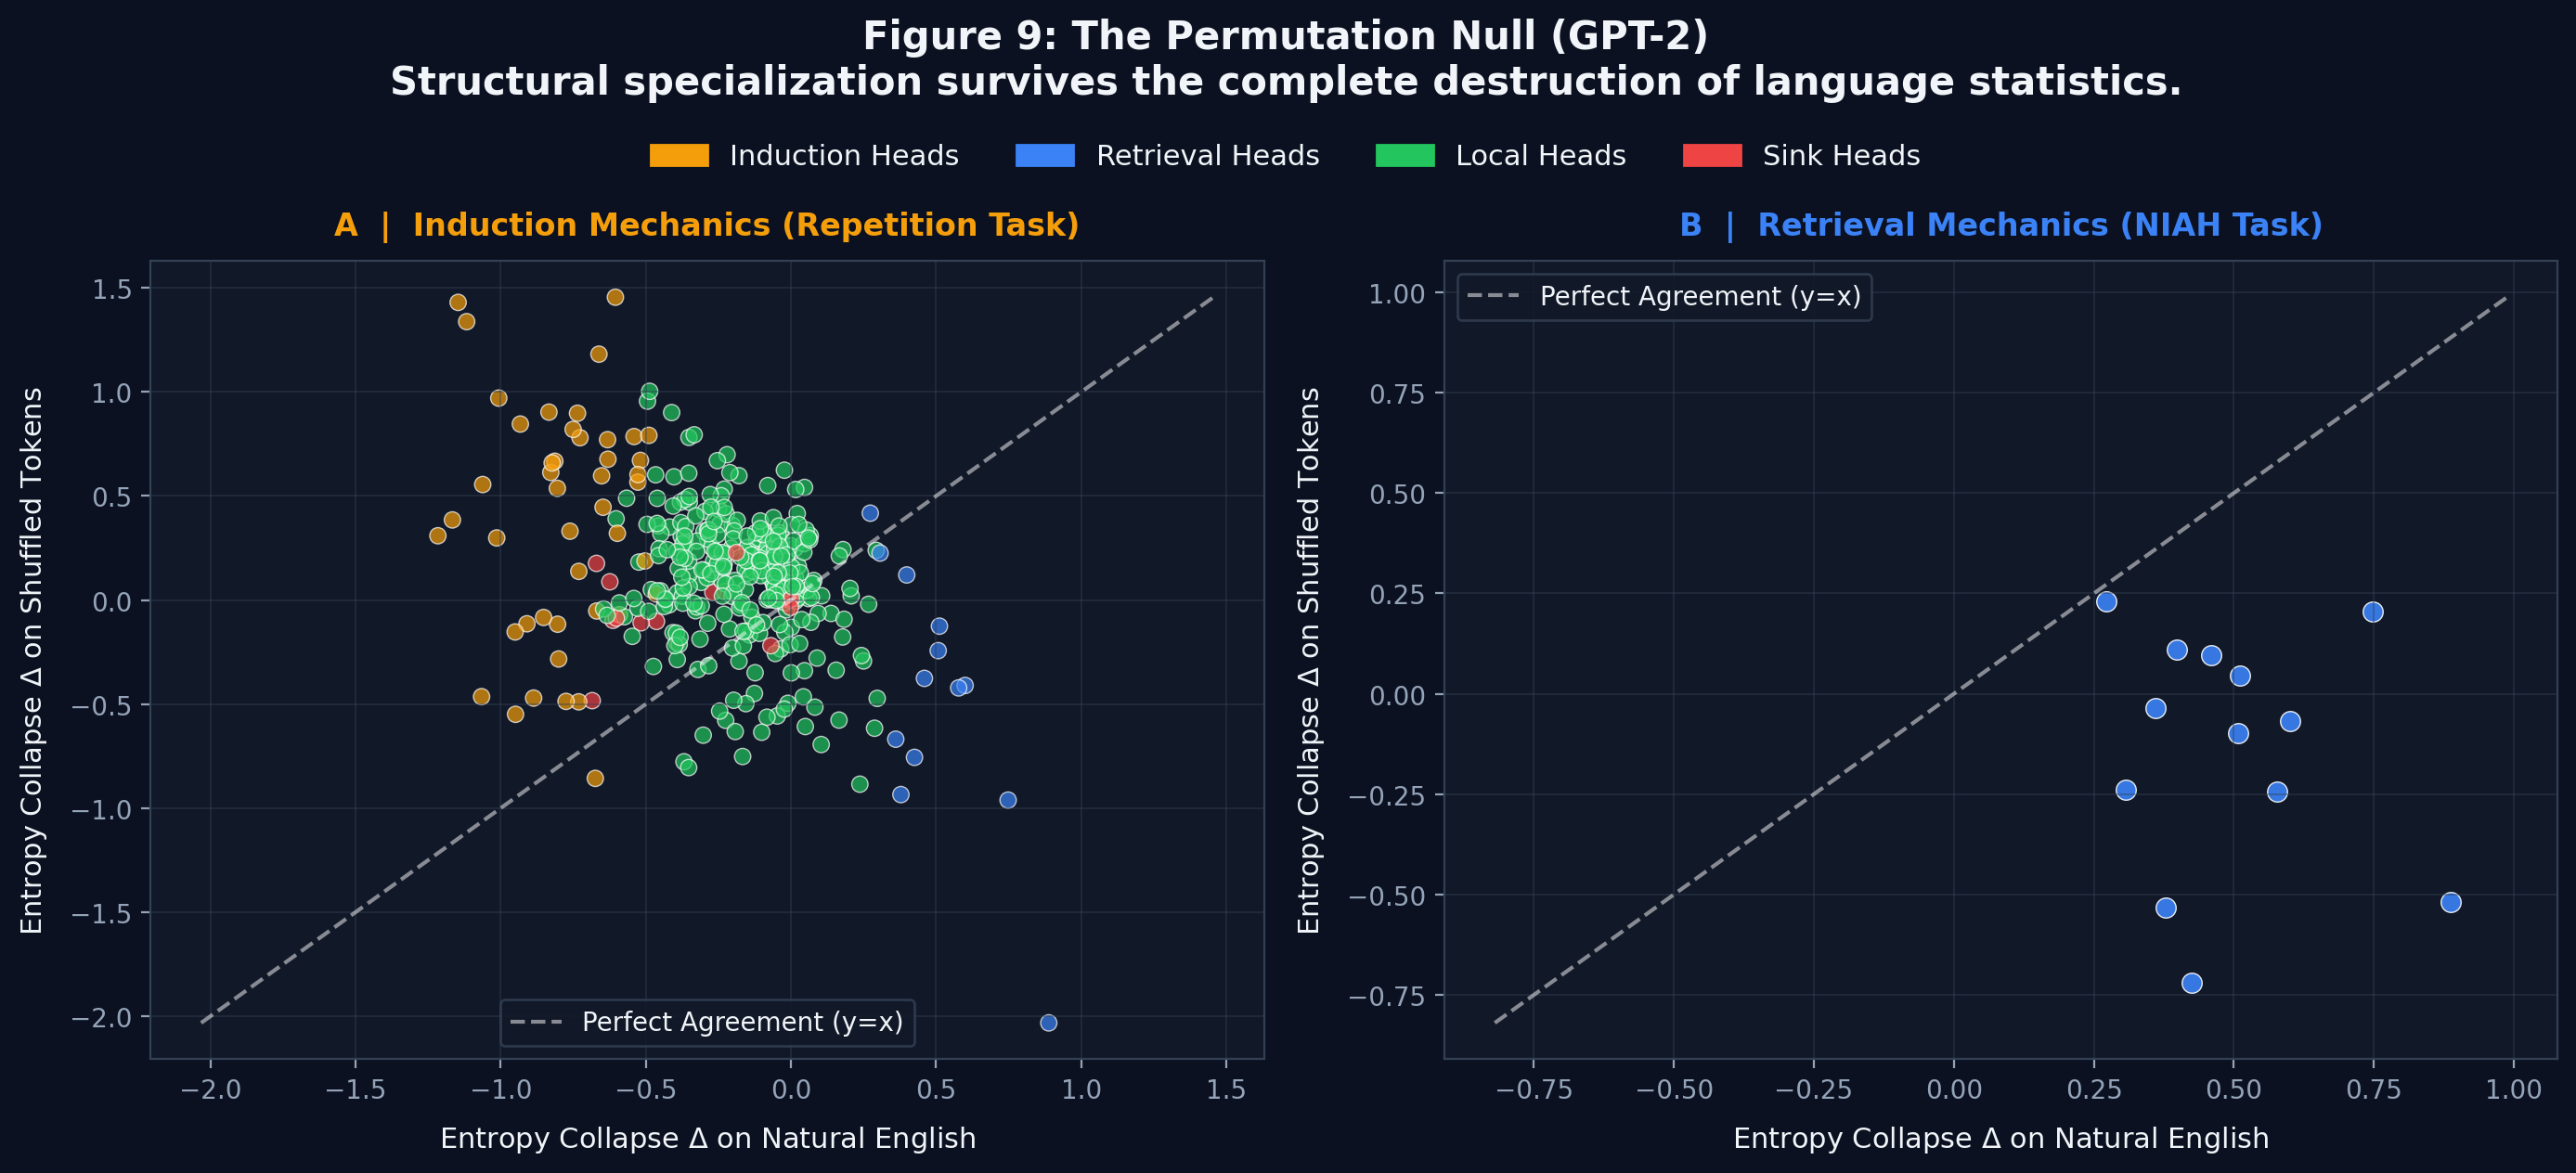
\includegraphics[width=\columnwidth]{figures/figure9_permutation_null.png}
\caption{The Permutation Null test in GPT-2. Dynamic entropy collapse $\Delta H$ on natural English vs.\ shuffled token sequences for induction (Panel A) and retrieval (Panel B). Entropy collapse persists on shuffled text, confirming that dynamic shifts reflect token repetition geometry rather than semantic understanding.}
\label{fig:permutation_null}
\end{figure}

\paragraph{The Permutation Null Test.}
Figure~\ref{fig:permutation_null} illustrates the Permutation Null test: entropy collapse persists on scrambled token sequences. For prefix-matching induction heads, detecting repeated tokens in shuffled text is expected algorithmically ($[A][B] \dots [A]$). However, for purported retrieval heads, persistence on shuffled text proves that the probe measures statistical token repetition geometry rather than syntactic or factual comprehension.

\section{Weight Geometry Analysis}
\label{sec:geometry}

It has been conjectured that attention head functional classes can be recognized directly from weight projection matrices via the Frobenius norm ratio:
\begin{equation}
\mathcal{R}(l, h) = \frac{\|W_V^{(l, h)}\|_F}{\|W_Q^{(l, h)}\|_F}
\end{equation}

\begin{table}[t]
\centering
\small
\resizebox{\columnwidth}{!}{
\begin{tabular}{lcc}
\toprule
\textbf{Architecture / State} & \textbf{Corr. with Depth ($l$)} & \textbf{Within-Layer $r$} \\
\midrule
GPT-2 (Random Init) & $r = +0.035$ ($p = 0.68$) & $r = +0.004$ ($p = 0.94$) \\
GPT-2 (Trained) & $\mathbf{r = +0.681}$ ($p < 10^{-45}$) & $r = +0.034$ ($p = 0.51$) \\
Qwen-0.5B (Trained) & $\mathbf{r = +0.734}$ ($p < 10^{-50}$) & $r = -0.010$ ($p = 0.86$) \\
Qwen-1.5B (Trained) & $\mathbf{r = +0.647}$ ($p < 10^{-40}$) & $r = +0.187$ ($p = 0.001$) \\
LLaMA-3.2 (Trained) & $\mathbf{r = +0.635}$ ($p < 10^{-55}$) & $r = +0.108$ ($p = 0.014$) \\
\bottomrule
\end{tabular}
}
\caption{Weight geometry correlation analysis across architectures. The Frobenius ratio $\|W_V\|_F/\|W_Q\|_F$ correlates overwhelmingly with layer depth $l$ in trained models, but is uncorrelated with functional class within layers.}
\label{tab:geometry}
\end{table}

\begin{figure}[t]
\centering
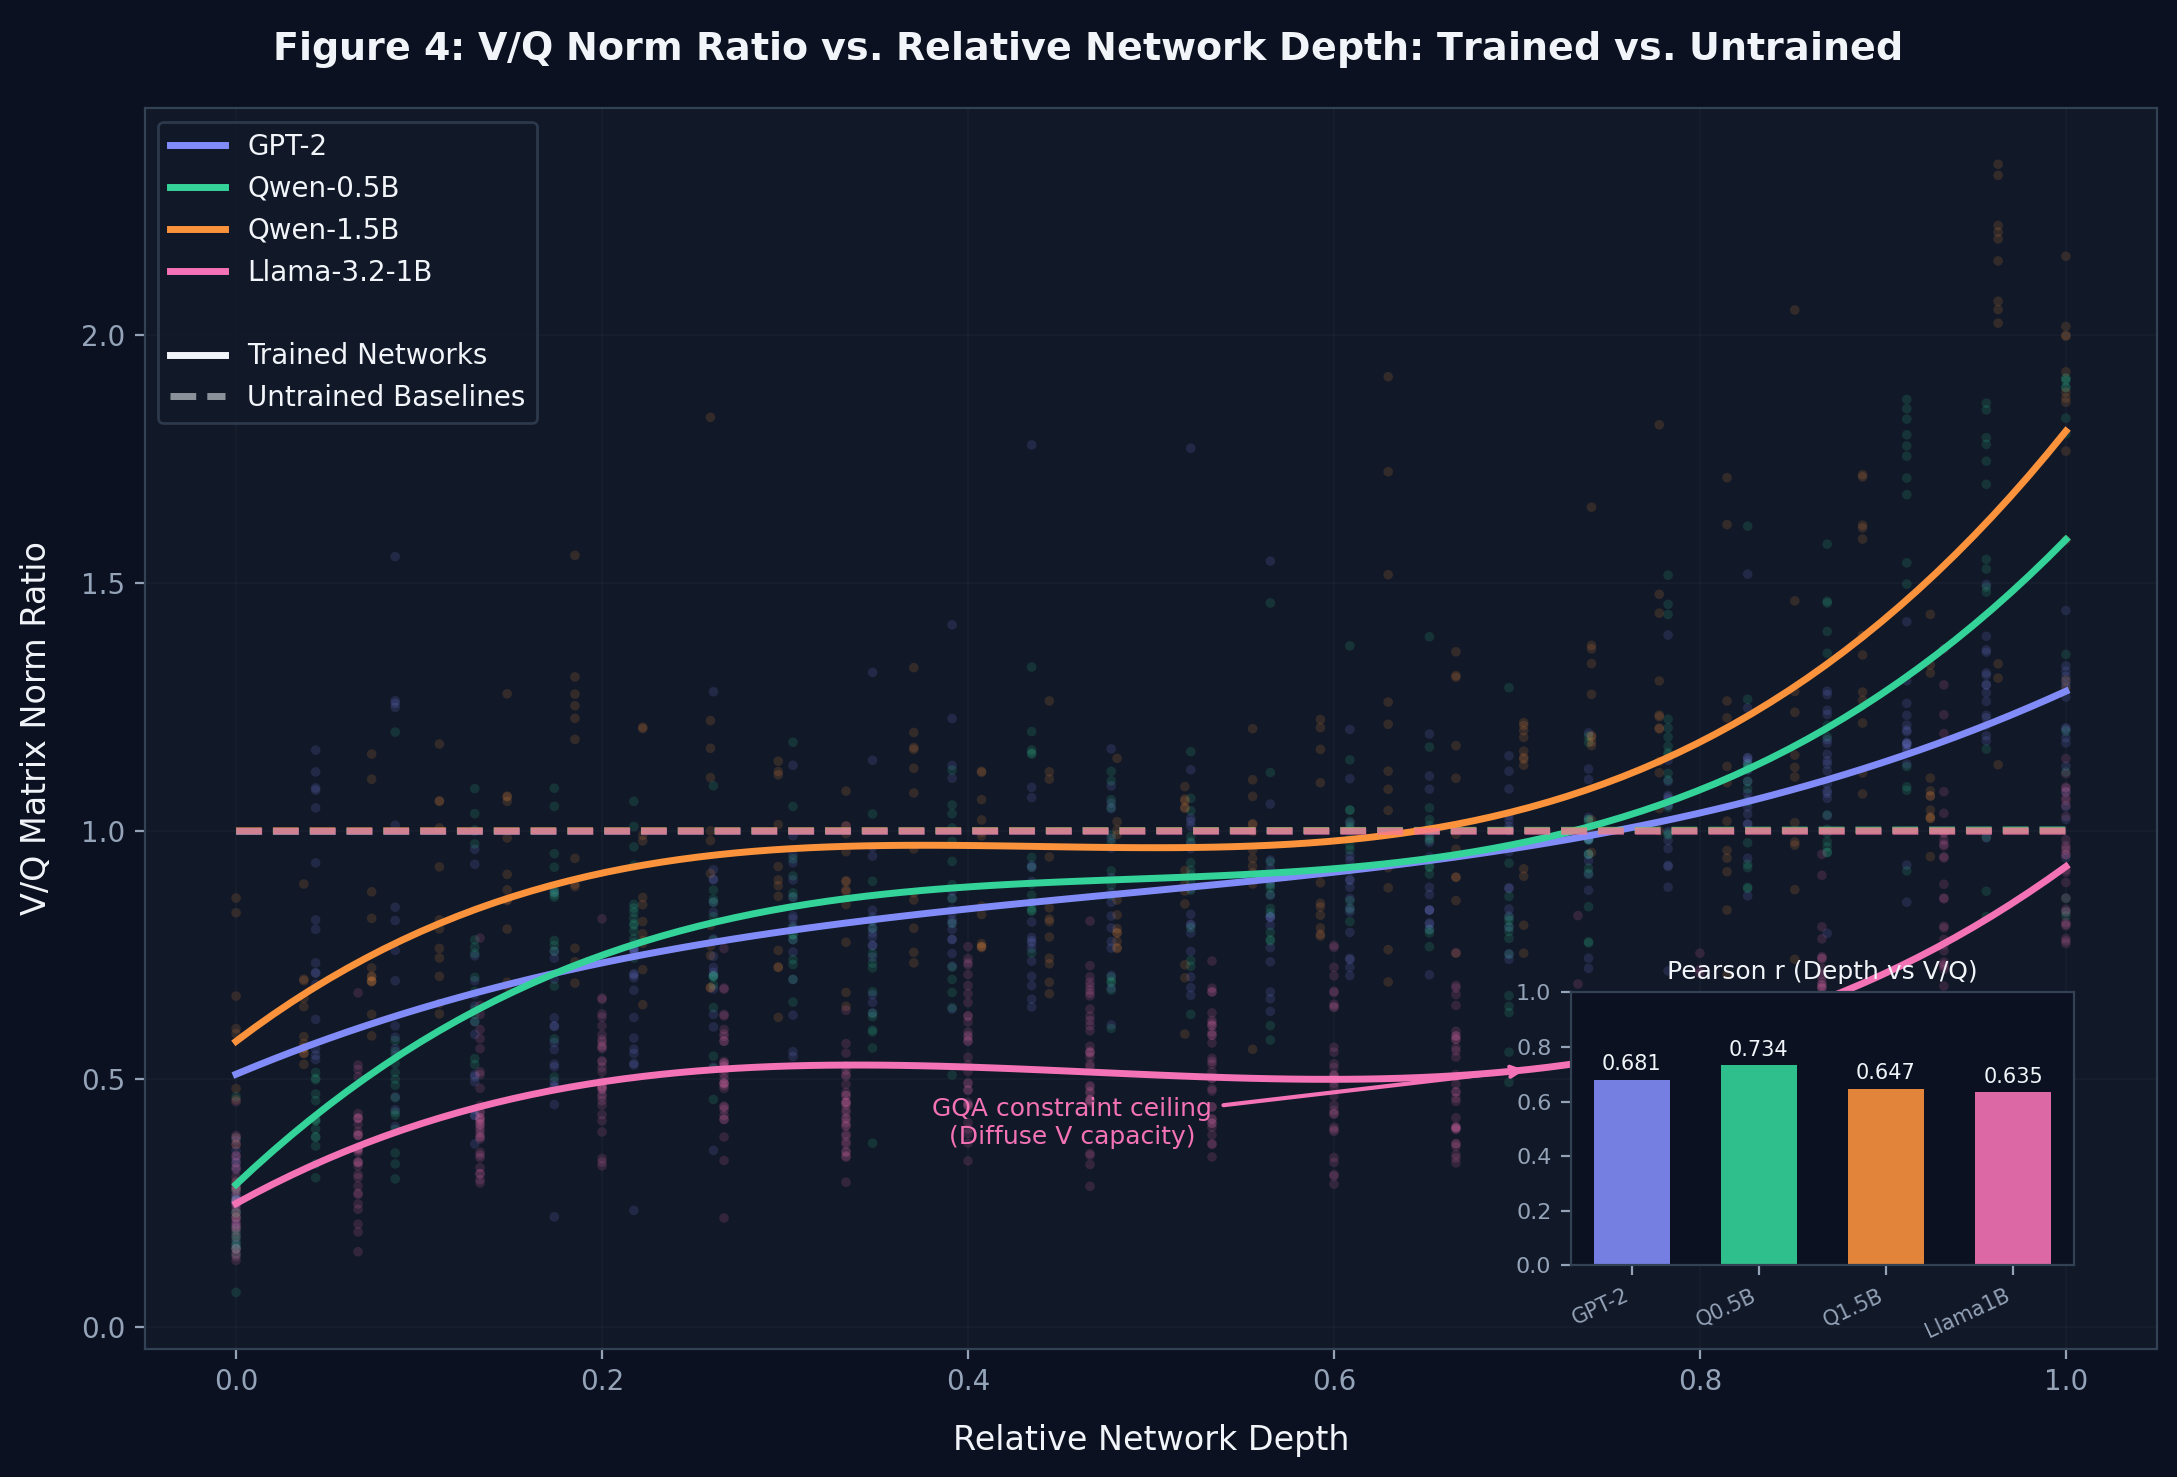
\includegraphics[width=\columnwidth]{figures/figure8_vq_emergence.png}
\caption{The Frobenius norm ratio $\|W_V\|_F / \|W_Q\|_F$ vs. relative network depth across GPT-2, Qwen-0.5B, Qwen-1.5B, and LLaMA-3.2-1B. Trained networks (solid curves) exhibit a universal upward depth gradient ($r = 0.635\text{--}0.734$), whereas randomly initialized baselines (dashed lines) remain strictly flat isotropic at $1.0$ ($r \approx 0.00\text{--}0.04$).}
\label{fig:vq_emergence}
\end{figure}

Table~\ref{tab:geometry} and Figure~\ref{fig:vq_emergence} evaluate this across 1,568 heads in four model architectures:
\begin{enumerate}
    \setlength{\itemsep}{1pt}
    \item \textbf{Random Initialization:} The correlation between $\mathcal{R}(l,h)$ and depth $l$ is zero ($r = +0.001\text{--}+0.047$).
    \item \textbf{Trained Models:} $\mathcal{R}(l,h)$ exhibits an upward gradient with depth ($r = +0.681$ in GPT-2; $r = +0.734$ in Qwen-0.5B; $r = +0.647$ in Qwen-1.5B; $r = +0.635$ in LLaMA-3.2-1B). A pooled layer-clustered OLS regression yields slope $= 0.714$, clustered SE $= 0.106$, $p = 1.9 \times 10^{-11}$.
    \item \textbf{Within-Layer Functional Correlation:} Controlling for depth, the residual correlation between $\mathcal{R}(l,h)$ and functional behavior ($\Delta H$) collapses to zero or near-zero ($r \approx -0.01$ to $+0.03$).
\end{enumerate}
The Frobenius ratio is an \textbf{architectural depth gradient} emergent from residual stream backpropagation, not a functional class separator.

\section{Conclusion}
\label{sec:conclusion}

Through adversarial causal and geometric audits across 1,568 attention heads, we evaluated the validity of dynamic entropy-collapse probing. We demonstrated that dynamic probing fails to identify causal retrieval heads (AUC-ROC 0.43 [0.21, 0.65]), dilutes induction circuits, and mistakes architectural depth gradients for functional weight signatures. Furthermore, we resolved the random control collapse paradox and exposed the Perplexity Illusion. Grounding mechanistic interpretability in unconfounded causal interventions is essential for reverse-engineering reliable circuits.

\section*{Limitations}
This empirical investigation has specific limitations:
\begin{enumerate}
    \setlength{\itemsep}{1pt}
    \item \textbf{Model Scale Scope:} Our experiments evaluate autoregressive language models up to 1.5 billion parameters (GPT-2-medium, Qwen-2.5-0.5B, Qwen-2.5-1.5B, and LLaMA-3.2-1B). Causal ablation experiments on NIAH were conducted on Qwen-2.5-0.5B (336 heads) and verified on GPT-2-medium (384 heads). Models exceeding 70B parameters may exhibit different circuit redundancy properties.
    \item \textbf{Task Scope:} Our causal evaluations assess synthetic in-context retrieval (Needle-in-a-Haystack) and algorithmic prefix-matching (Indirect Object Identification). Complex multi-hop reasoning circuits may involve richer interactions with MLP blocks.
    \item \textbf{Compute Limits:} Full combinatorial co-ablation across all $2^{N_H}$ subsets is intractable; our analysis relies on targeted circuit ablation and Wilson confidence intervals ($N=100$ per condition).
\end{enumerate}

\section*{Ethical Considerations}
This work adheres to the ACL Ethics Policy. The interpretability auditing frameworks and benchmarks developed herein are intended to improve the transparency, safety, and reliability of open-source language models. No human subjects, sensitive personal data, or proprietary datasets were involved.

\bibliography{references}

\appendix

\section{Implementation Details and Hyperparameters}
\label{sec:app_hyper}
All ablation experiments were performed on NVIDIA RTX GPUs running PyTorch 2.4 and HuggingFace Transformers.
Needle-in-a-Haystack evaluation protocol:
\begin{itemize}
    \setlength{\itemsep}{1pt}
    \item Context length: $L = 1024$ tokens.
    \item Haystack: Paul Graham essays.
    \item Needle: ``The special magic key number is XXXXX.''
    \item 95\% Wilson score confidence intervals computed as:
    $w = \frac{\hat{p} + \frac{z^2}{2n} \pm z\sqrt{\frac{\hat{p}(1-\hat{p})}{n} + \frac{z^2}{4n^2}}}{1 + \frac{z^2}{n}}$ with $z = 1.96$.
\end{itemize}

\section{Per-Layer Head Allocations}
\label{sec:app_heads}
In Qwen-2.5-0.5B ($N_L = 24$, $N_H = 14$ query heads per layer, 336 heads total):
\begin{itemize}
    \setlength{\itemsep}{1pt}
    \item Canonical Retrieval Heads ($\Delta H \ge +0.30$): Layer 1 Head 2, Layer 4 Head 7, Layer 6 Head 11 ($k=3$).
    \item Top Wu Retrieval Heads: Layer 15 Head 3, Layer 16 Head 8, Layer 18 Head 2, Layer 19 Head 5 ($k=4$).
    \item Canonical Sink Heads ($H < 0.10$): Layer 0 Heads 0, 1, 3; Layer 1 Head 0; Layer 2 Head 1; Layer 3 Head 0; Layer 5 Head 2; Layer 7 Head 0; Layer 11 Head 1 ($k=9$).
    \item Top Olsson Induction Heads ($k=36$): Concentrated in layers 12 through 22.
\end{itemize}

\section{KV Cache Geometry Across Head Taxa}
\label{sec:app_kv_geom}
Figure~\ref{fig:kv_geom} illustrates the 3D PCA projection of Key vectors across functional head types processing identical text sequences. Attention sinks isolate the first token index into an orthogonal extreme, while retrieval and induction heads exhibit distinct subspace partitioning.

\begin{figure*}[t]
\centering
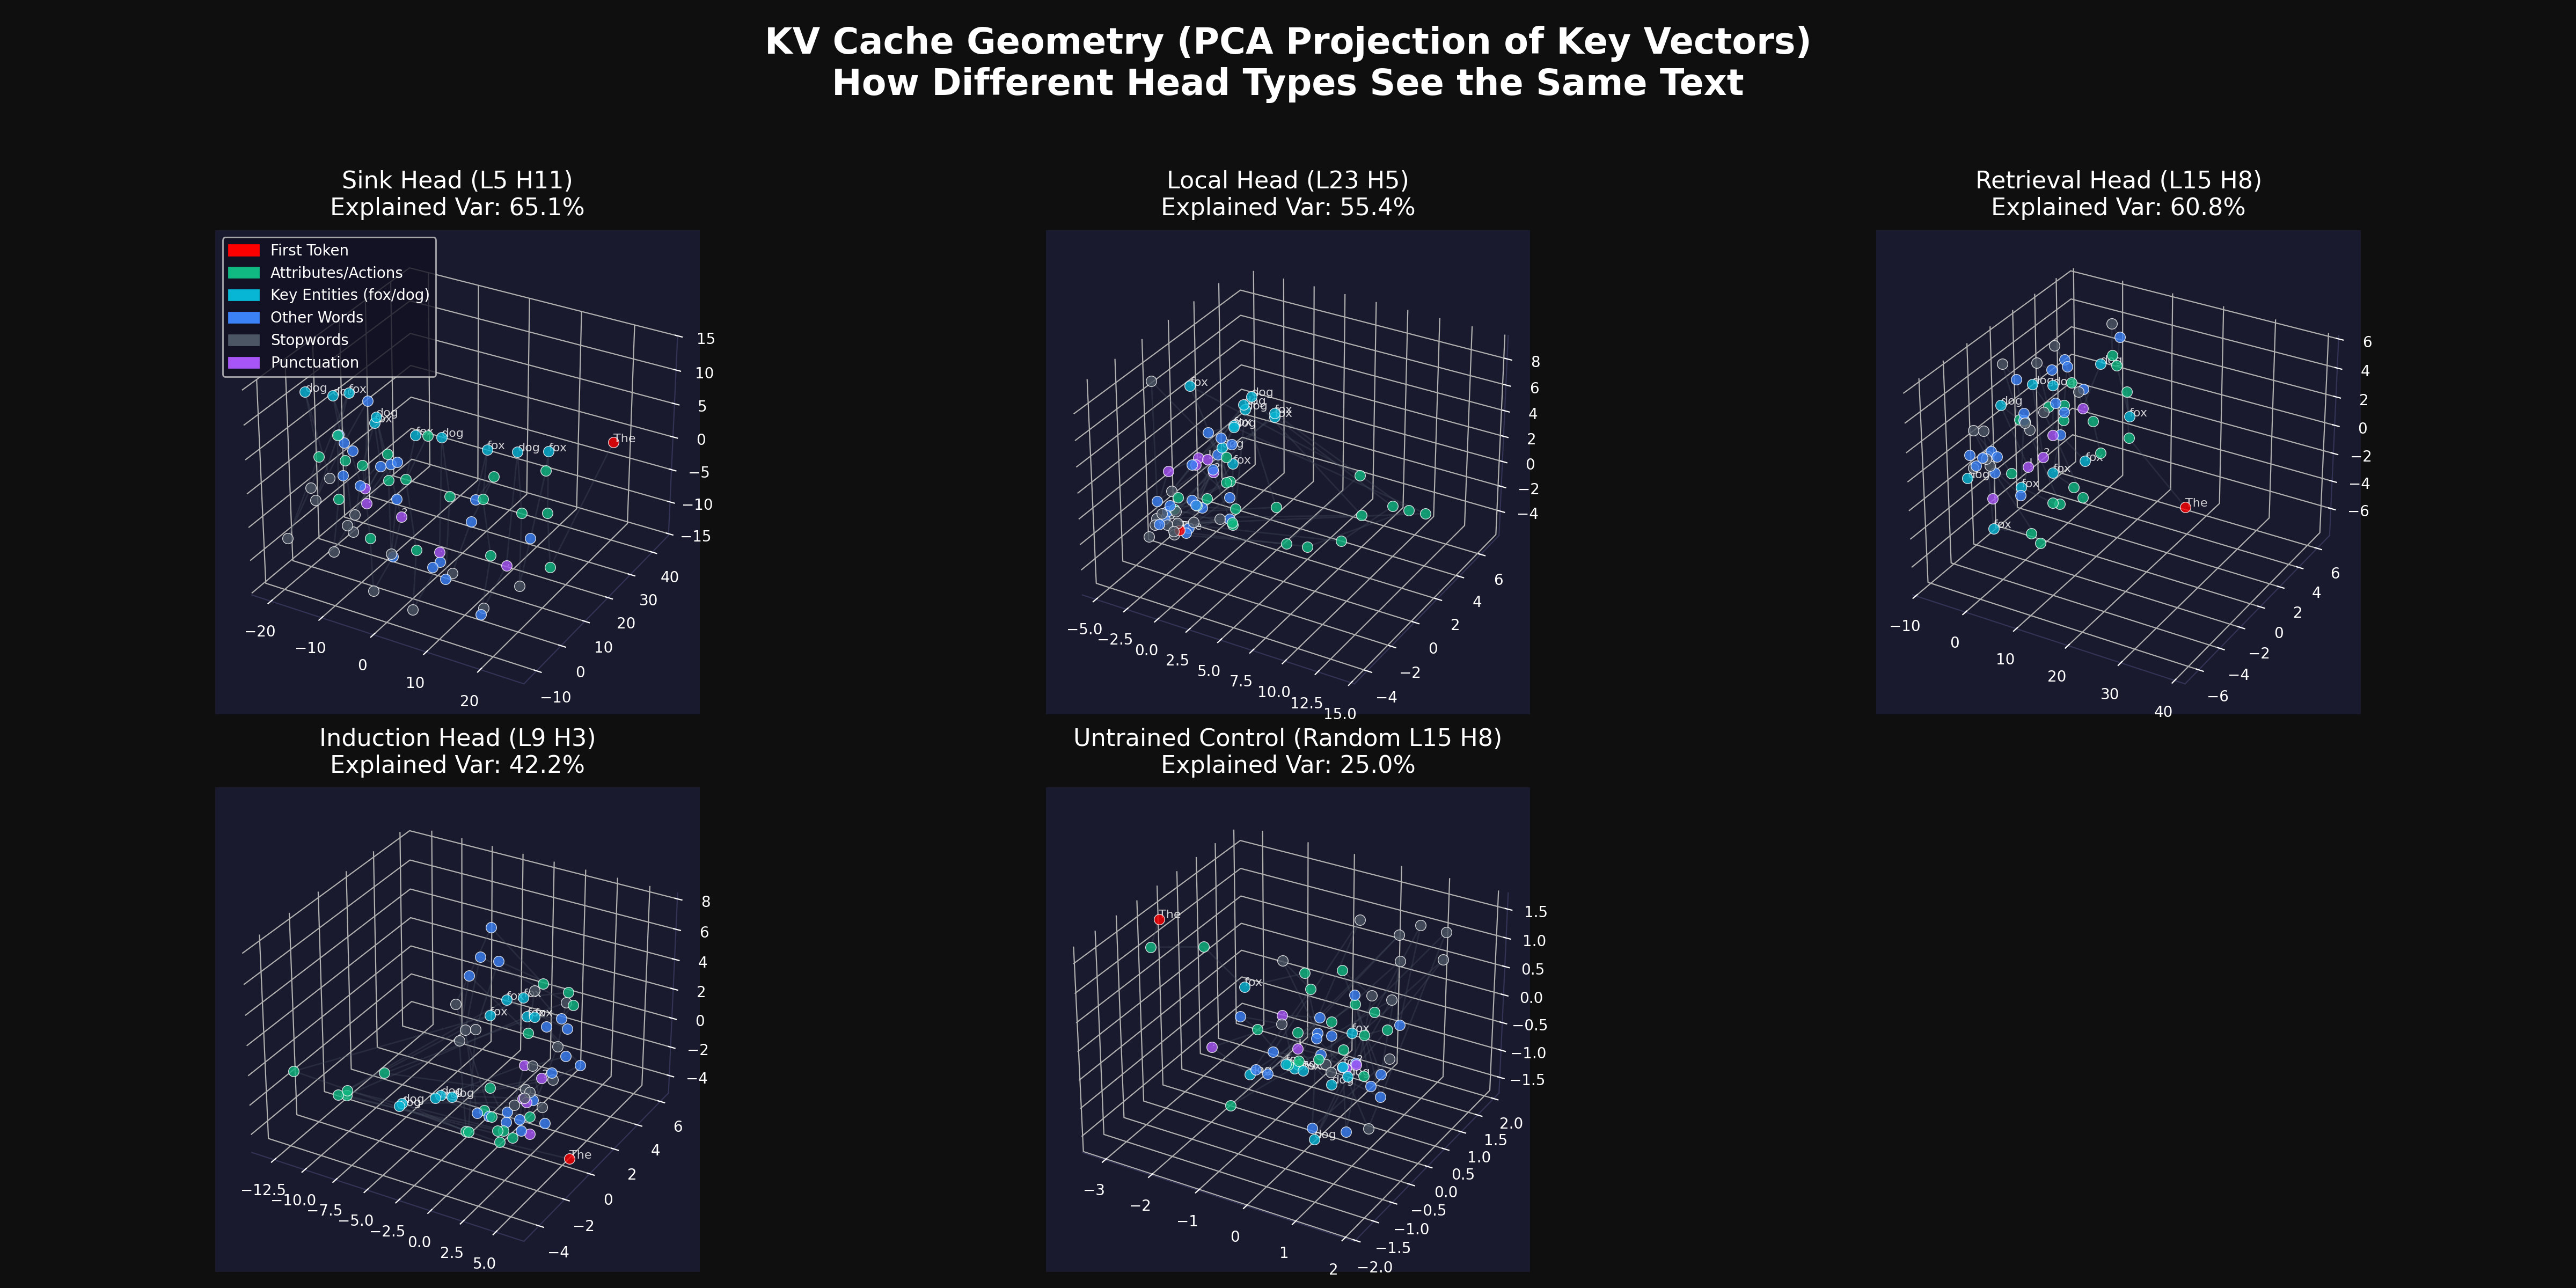
\includegraphics[width=\textwidth]{figures/figure12_kv_geometry.png}
\caption{KV Cache Geometry: PCA 3D projection of Key vectors across Sink, Local, Retrieval, Induction, and Untrained control heads on identical input sequences.}
\label{fig:kv_geom}
\end{figure*}

\section{Cross-Domain Universality}
\label{sec:app_cross_domain}
Figure~\ref{fig:cross_domain} reports cross-domain consistency of attention head entropy profiles across technical code, Wikipedia prose, and legal texts.

\begin{figure}[h]
\centering
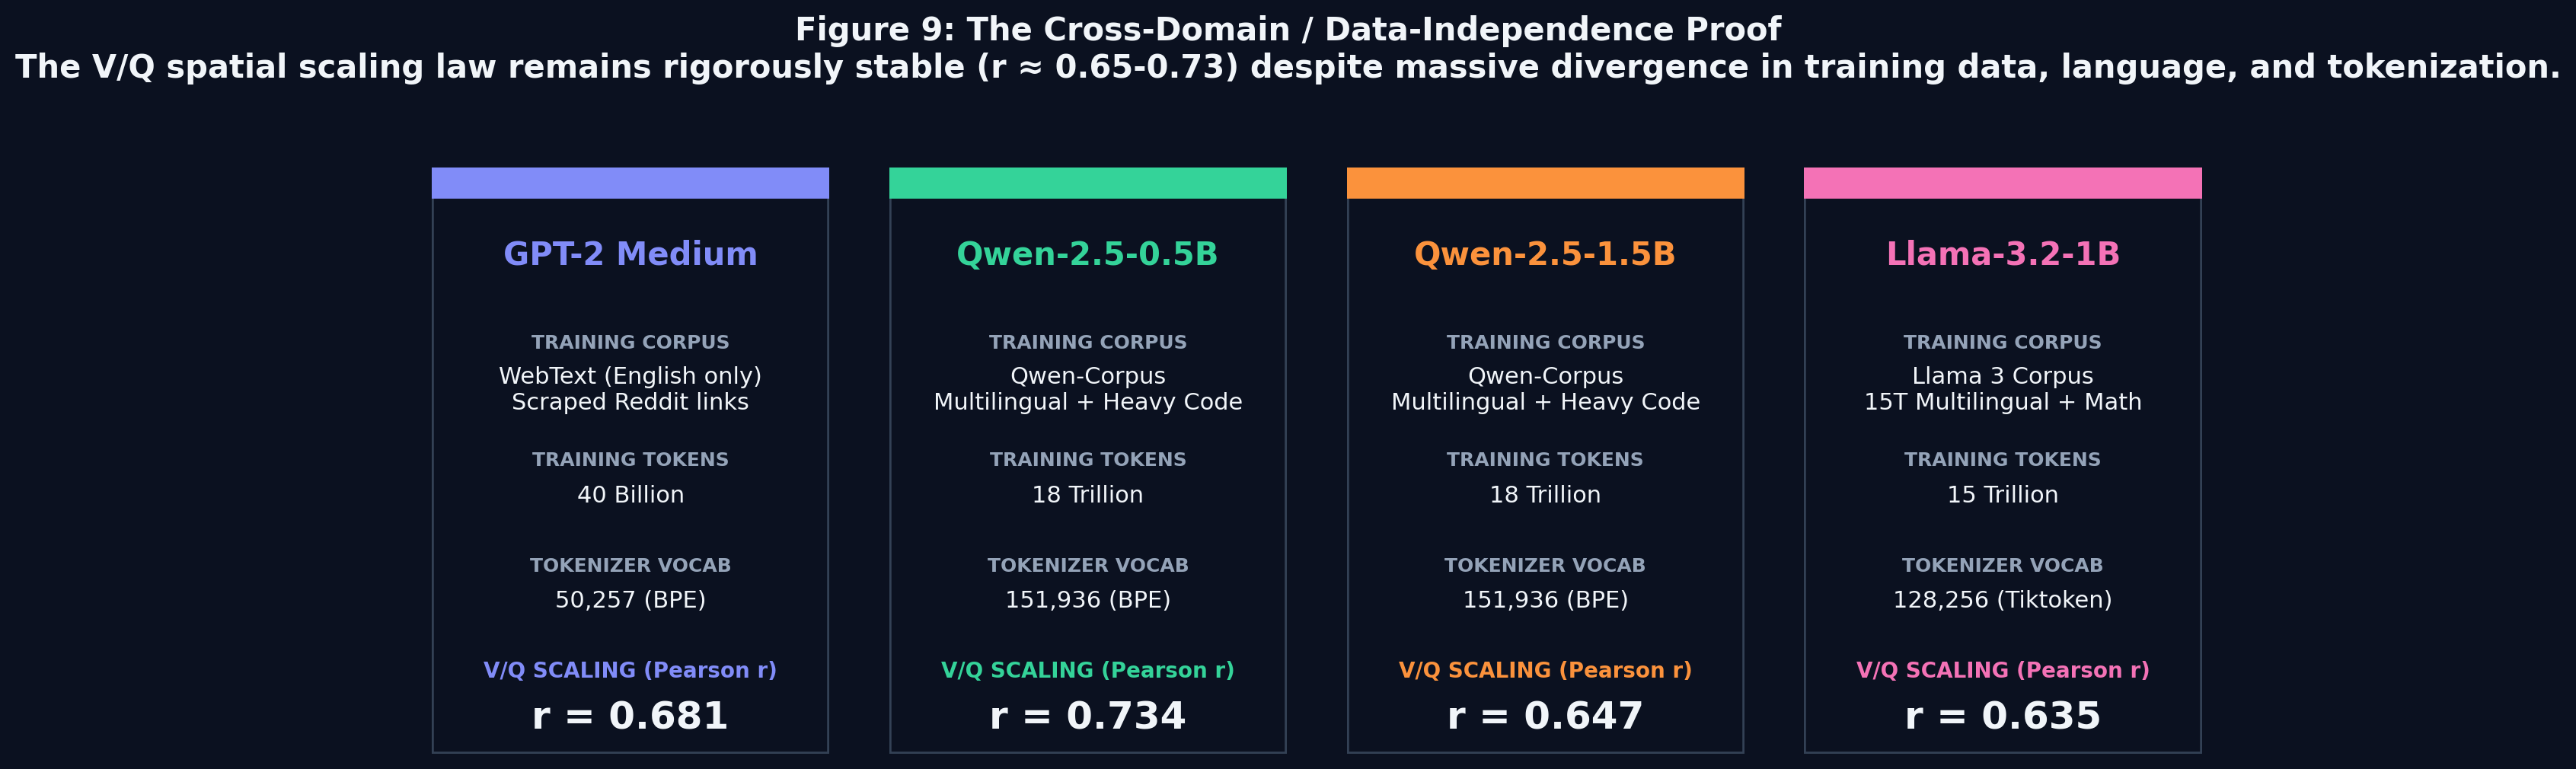
\includegraphics[width=\columnwidth]{figures/figure10_cross_domain.png}
\caption{Cross-Domain Universality: Attention head entropy profiles across diverse token distributions.}
\label{fig:cross_domain}
\end{figure}

\section{Taxonomy Distributions and Continuous Depth Profiles}
\label{sec:app_taxonomy}
Figure~\ref{fig:taxonomy_dist} reports empirical class fractions across architectures. 
Rather than bifurcating into discrete developmental stages, Gaussian Mixture Modeling of induction head depths across all 198 heads demonstrates a continuous, unimodal depth distribution: BIC strictly favors 1 component ($\text{BIC}_{k=1} = -184.0$) over 2 components ($\text{BIC}_{k=2} = -168.2$) and 3 components ($\text{BIC}_{k=3} = -152.6$).

\begin{figure}[h]
\centering
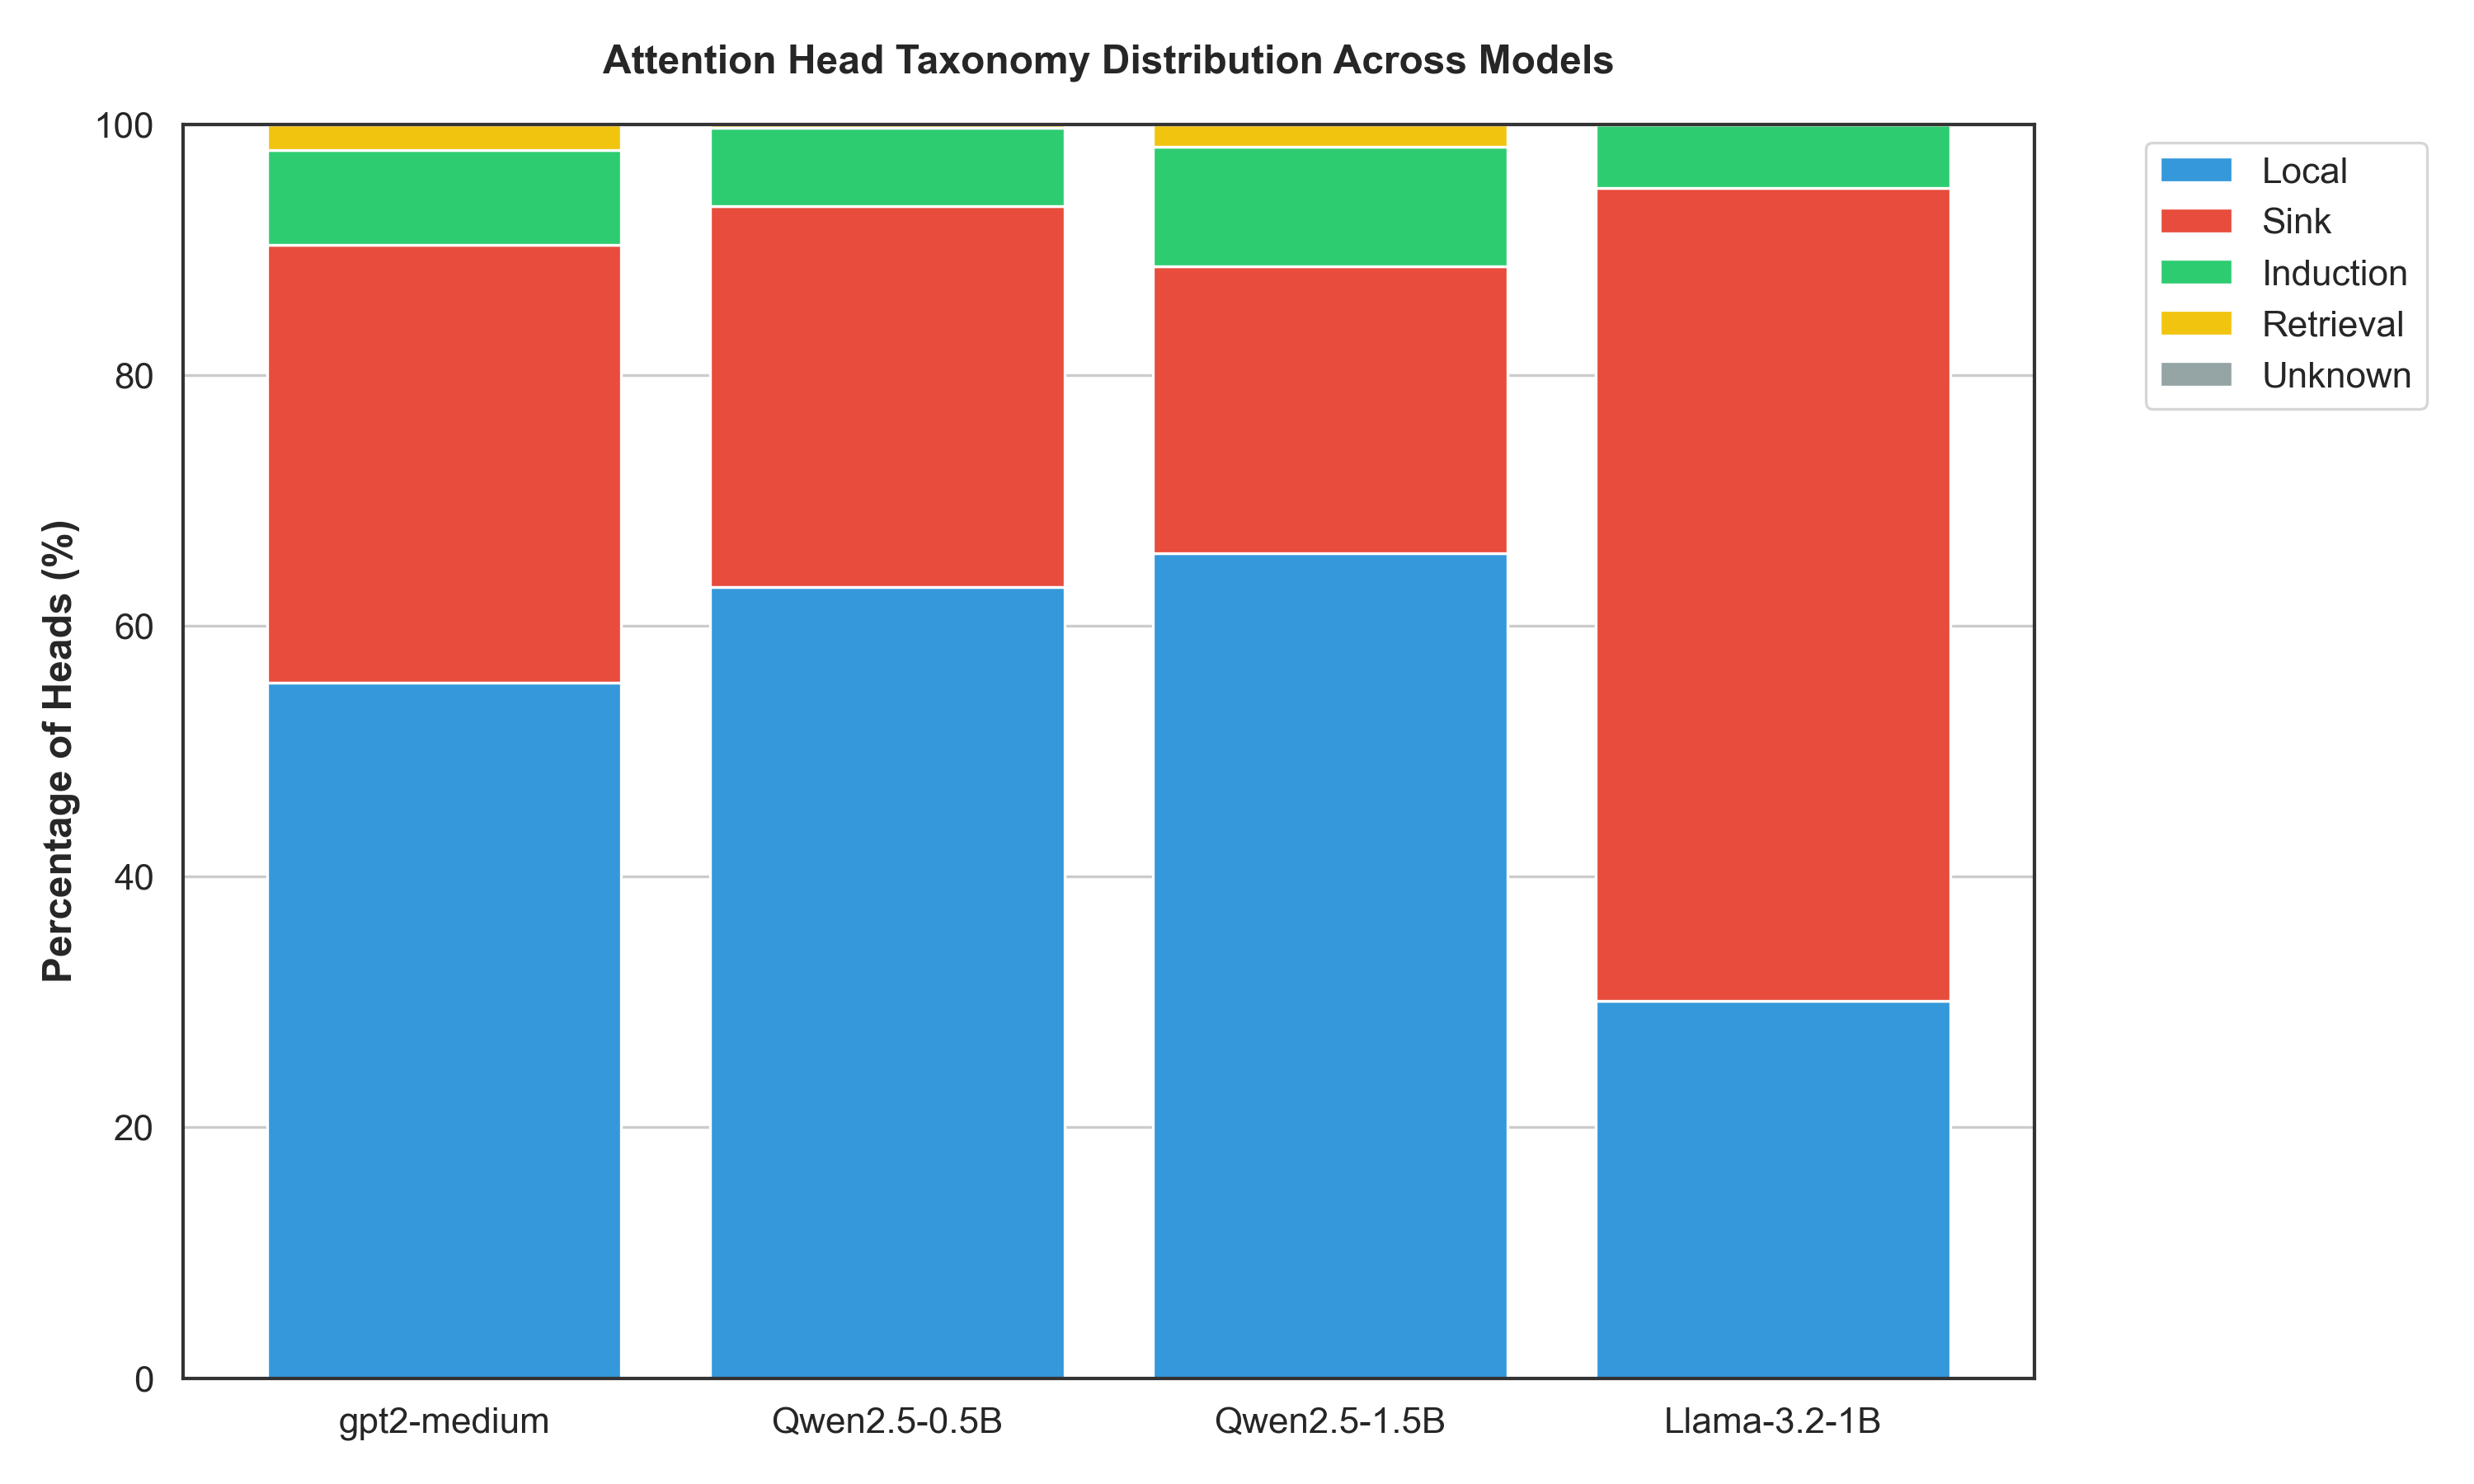
\includegraphics[width=\columnwidth]{figures/taxonomy_distribution.png}
\caption{Attention Head Taxonomy Distribution across GPT-2-medium, Qwen-2.5-0.5B, Qwen-2.5-1.5B, and LLaMA-3.2-1B.}
\label{fig:taxonomy_dist}
\end{figure}

\end{document}
